\PassOptionsToPackage{unicode=true}{hyperref} % options for packages loaded elsewhere
\PassOptionsToPackage{hyphens}{url}
%
\documentclass[]{article}
\usepackage{lmodern}
\usepackage{amssymb,amsmath}
\usepackage{ifxetex,ifluatex}
\usepackage{fixltx2e} % provides \textsubscript
\ifnum 0\ifxetex 1\fi\ifluatex 1\fi=0 % if pdftex
  \usepackage[T1]{fontenc}
  \usepackage[utf8]{inputenc}
  \usepackage{textcomp} % provides euro and other symbols
\else % if luatex or xelatex
  \usepackage{unicode-math}
  \defaultfontfeatures{Ligatures=TeX,Scale=MatchLowercase}
\fi
% use upquote if available, for straight quotes in verbatim environments
\IfFileExists{upquote.sty}{\usepackage{upquote}}{}
% use microtype if available
\IfFileExists{microtype.sty}{%
\usepackage[]{microtype}
\UseMicrotypeSet[protrusion]{basicmath} % disable protrusion for tt fonts
}{}
\IfFileExists{parskip.sty}{%
\usepackage{parskip}
}{% else
\setlength{\parindent}{0pt}
\setlength{\parskip}{6pt plus 2pt minus 1pt}
}
\usepackage{hyperref}
\hypersetup{
            pdftitle={Quantification of AMPK Knockout Blots},
            pdfauthor={Dave Bridges},
            pdfborder={0 0 0},
            breaklinks=true}
\urlstyle{same}  % don't use monospace font for urls
\usepackage[margin=1in]{geometry}
\usepackage{color}
\usepackage{fancyvrb}
\newcommand{\VerbBar}{|}
\newcommand{\VERB}{\Verb[commandchars=\\\{\}]}
\DefineVerbatimEnvironment{Highlighting}{Verbatim}{commandchars=\\\{\}}
% Add ',fontsize=\small' for more characters per line
\usepackage{framed}
\definecolor{shadecolor}{RGB}{248,248,248}
\newenvironment{Shaded}{\begin{snugshade}}{\end{snugshade}}
\newcommand{\AlertTok}[1]{\textcolor[rgb]{0.94,0.16,0.16}{#1}}
\newcommand{\AnnotationTok}[1]{\textcolor[rgb]{0.56,0.35,0.01}{\textbf{\textit{#1}}}}
\newcommand{\AttributeTok}[1]{\textcolor[rgb]{0.77,0.63,0.00}{#1}}
\newcommand{\BaseNTok}[1]{\textcolor[rgb]{0.00,0.00,0.81}{#1}}
\newcommand{\BuiltInTok}[1]{#1}
\newcommand{\CharTok}[1]{\textcolor[rgb]{0.31,0.60,0.02}{#1}}
\newcommand{\CommentTok}[1]{\textcolor[rgb]{0.56,0.35,0.01}{\textit{#1}}}
\newcommand{\CommentVarTok}[1]{\textcolor[rgb]{0.56,0.35,0.01}{\textbf{\textit{#1}}}}
\newcommand{\ConstantTok}[1]{\textcolor[rgb]{0.00,0.00,0.00}{#1}}
\newcommand{\ControlFlowTok}[1]{\textcolor[rgb]{0.13,0.29,0.53}{\textbf{#1}}}
\newcommand{\DataTypeTok}[1]{\textcolor[rgb]{0.13,0.29,0.53}{#1}}
\newcommand{\DecValTok}[1]{\textcolor[rgb]{0.00,0.00,0.81}{#1}}
\newcommand{\DocumentationTok}[1]{\textcolor[rgb]{0.56,0.35,0.01}{\textbf{\textit{#1}}}}
\newcommand{\ErrorTok}[1]{\textcolor[rgb]{0.64,0.00,0.00}{\textbf{#1}}}
\newcommand{\ExtensionTok}[1]{#1}
\newcommand{\FloatTok}[1]{\textcolor[rgb]{0.00,0.00,0.81}{#1}}
\newcommand{\FunctionTok}[1]{\textcolor[rgb]{0.00,0.00,0.00}{#1}}
\newcommand{\ImportTok}[1]{#1}
\newcommand{\InformationTok}[1]{\textcolor[rgb]{0.56,0.35,0.01}{\textbf{\textit{#1}}}}
\newcommand{\KeywordTok}[1]{\textcolor[rgb]{0.13,0.29,0.53}{\textbf{#1}}}
\newcommand{\NormalTok}[1]{#1}
\newcommand{\OperatorTok}[1]{\textcolor[rgb]{0.81,0.36,0.00}{\textbf{#1}}}
\newcommand{\OtherTok}[1]{\textcolor[rgb]{0.56,0.35,0.01}{#1}}
\newcommand{\PreprocessorTok}[1]{\textcolor[rgb]{0.56,0.35,0.01}{\textit{#1}}}
\newcommand{\RegionMarkerTok}[1]{#1}
\newcommand{\SpecialCharTok}[1]{\textcolor[rgb]{0.00,0.00,0.00}{#1}}
\newcommand{\SpecialStringTok}[1]{\textcolor[rgb]{0.31,0.60,0.02}{#1}}
\newcommand{\StringTok}[1]{\textcolor[rgb]{0.31,0.60,0.02}{#1}}
\newcommand{\VariableTok}[1]{\textcolor[rgb]{0.00,0.00,0.00}{#1}}
\newcommand{\VerbatimStringTok}[1]{\textcolor[rgb]{0.31,0.60,0.02}{#1}}
\newcommand{\WarningTok}[1]{\textcolor[rgb]{0.56,0.35,0.01}{\textbf{\textit{#1}}}}
\usepackage{longtable,booktabs}
% Fix footnotes in tables (requires footnote package)
\IfFileExists{footnote.sty}{\usepackage{footnote}\makesavenoteenv{longtable}}{}
\usepackage{graphicx,grffile}
\makeatletter
\def\maxwidth{\ifdim\Gin@nat@width>\linewidth\linewidth\else\Gin@nat@width\fi}
\def\maxheight{\ifdim\Gin@nat@height>\textheight\textheight\else\Gin@nat@height\fi}
\makeatother
% Scale images if necessary, so that they will not overflow the page
% margins by default, and it is still possible to overwrite the defaults
% using explicit options in \includegraphics[width, height, ...]{}
\setkeys{Gin}{width=\maxwidth,height=\maxheight,keepaspectratio}
\setlength{\emergencystretch}{3em}  % prevent overfull lines
\providecommand{\tightlist}{%
  \setlength{\itemsep}{0pt}\setlength{\parskip}{0pt}}
\setcounter{secnumdepth}{5}
% Redefines (sub)paragraphs to behave more like sections
\ifx\paragraph\undefined\else
\let\oldparagraph\paragraph
\renewcommand{\paragraph}[1]{\oldparagraph{#1}\mbox{}}
\fi
\ifx\subparagraph\undefined\else
\let\oldsubparagraph\subparagraph
\renewcommand{\subparagraph}[1]{\oldsubparagraph{#1}\mbox{}}
\fi

% set default figure placement to htbp
\makeatletter
\def\fps@figure{htbp}
\makeatother


\title{Quantification of AMPK Knockout Blots}
\author{Dave Bridges}
\date{June 18, 2020}

\begin{document}
\maketitle

{
\setcounter{tocdepth}{2}
\tableofcontents
}
\hypertarget{purpose}{%
\section{Purpose}\label{purpose}}

\hypertarget{experimental-details}{%
\section{Experimental Details}\label{experimental-details}}

Blotted liver lysates for AMPK and ACC

\hypertarget{raw-data}{%
\section{Raw Data}\label{raw-data}}

These data can be found in \textbf{/Volumes/BridgesLab/Kistler/AMPK
KO/Blots/Katherine Blots July 2020/Quantification} in files named
\textbf{Male ACC.xls} and \textbf{Male pACC.xls}. This script was most
recently updated on \textbf{Thu Jul 16 14:09:00 2020}.

\hypertarget{analysis}{%
\section{Analysis}\label{analysis}}

\hypertarget{lipogenic-proteins}{%
\section{Lipogenic Proteins}\label{lipogenic-proteins}}

\hypertarget{fatty-acid-synthase}{%
\subsection{Fatty Acid Synthase}\label{fatty-acid-synthase}}

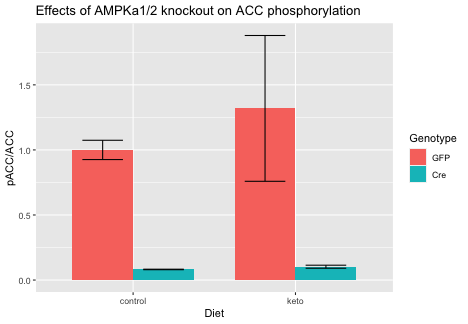
\includegraphics{figures/fas-barplot-1.png}

\begin{longtable}[]{@{}lrrrrr@{}}
\caption{ANOVA for FAS levels, no interaction}\tabularnewline
\toprule
term & df & sumsq & meansq & statistic & p.value\tabularnewline
\midrule
\endfirsthead
\toprule
term & df & sumsq & meansq & statistic & p.value\tabularnewline
\midrule
\endhead
Diet & 1 & 0 & 0 & 2.29 & 0.161\tabularnewline
Genotype & 1 & 0 & 0 & 0.02 & 0.889\tabularnewline
Residuals & 10 & 0 & 0 & NA & NA\tabularnewline
\bottomrule
\end{longtable}

\begin{longtable}[]{@{}lrrrrr@{}}
\caption{ANOVA for FAS levels, with interaction}\tabularnewline
\toprule
term & df & sumsq & meansq & statistic & p.value\tabularnewline
\midrule
\endfirsthead
\toprule
term & df & sumsq & meansq & statistic & p.value\tabularnewline
\midrule
\endhead
Diet & 1 & 0 & 0 & 2.209 & 0.171\tabularnewline
Genotype & 1 & 0 & 0 & 0.020 & 0.892\tabularnewline
Diet:Genotype & 1 & 0 & 0 & 0.642 & 0.443\tabularnewline
Residuals & 9 & 0 & 0 & NA & NA\tabularnewline
\bottomrule
\end{longtable}

\hypertarget{acetyl-coa-carboxylase}{%
\subsection{Acetyl-CoA Carboxylase}\label{acetyl-coa-carboxylase}}

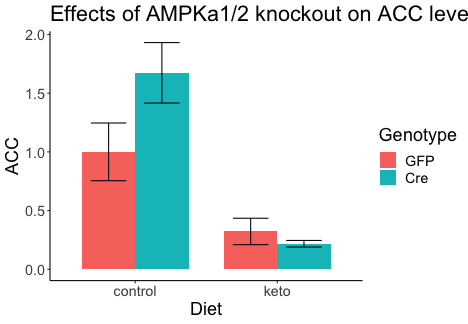
\includegraphics{figures/acc-barplot-1.png}

\begin{longtable}[]{@{}lrrrrr@{}}
\caption{ANOVA for ACC levels, no interaction}\tabularnewline
\toprule
term & df & sumsq & meansq & statistic & p.value\tabularnewline
\midrule
\endfirsthead
\toprule
term & df & sumsq & meansq & statistic & p.value\tabularnewline
\midrule
\endhead
Diet & 1 & 0 & 0 & 28.05 & 0.000\tabularnewline
Genotype & 1 & 0 & 0 & 1.62 & 0.232\tabularnewline
Residuals & 10 & 0 & 0 & NA & NA\tabularnewline
\bottomrule
\end{longtable}

\begin{longtable}[]{@{}lrrrrr@{}}
\caption{ANOVA for ACC levels, with interaction}\tabularnewline
\toprule
term & df & sumsq & meansq & statistic & p.value\tabularnewline
\midrule
\endfirsthead
\toprule
term & df & sumsq & meansq & statistic & p.value\tabularnewline
\midrule
\endhead
Diet & 1 & 0 & 0 & 39.70 & 0.000\tabularnewline
Genotype & 1 & 0 & 0 & 2.29 & 0.165\tabularnewline
Diet:Genotype & 1 & 0 & 0 & 5.15 & 0.049\tabularnewline
Residuals & 9 & 0 & 0 & NA & NA\tabularnewline
\bottomrule
\end{longtable}

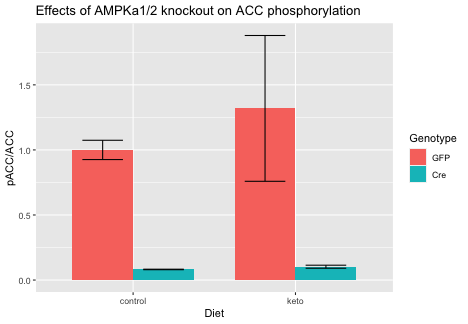
\includegraphics{figures/pACC-barplot-1.png}

\begin{longtable}[]{@{}lrrrrr@{}}
\caption{ANOVA for ACC phosphorylation, no interaction}\tabularnewline
\toprule
term & df & sumsq & meansq & statistic & p.value\tabularnewline
\midrule
\endfirsthead
\toprule
term & df & sumsq & meansq & statistic & p.value\tabularnewline
\midrule
\endhead
Diet & 1 & 0.305 & 0.305 & 0.112 & 0.744\tabularnewline
Genotype & 1 & 50.890 & 50.890 & 18.766 & 0.001\tabularnewline
Residuals & 10 & 27.118 & 2.712 & NA & NA\tabularnewline
\bottomrule
\end{longtable}

\begin{longtable}[]{@{}lrrrrr@{}}
\caption{ANOVA for ACC phosphorylation, with interaction}\tabularnewline
\toprule
term & df & sumsq & meansq & statistic & p.value\tabularnewline
\midrule
\endfirsthead
\toprule
term & df & sumsq & meansq & statistic & p.value\tabularnewline
\midrule
\endhead
Diet & 1 & 0.305 & 0.305 & 0.105 & 0.753\tabularnewline
Genotype & 1 & 50.890 & 50.890 & 17.515 & 0.002\tabularnewline
Diet:Genotype & 1 & 0.969 & 0.969 & 0.334 & 0.578\tabularnewline
Residuals & 9 & 26.149 & 2.905 & NA & NA\tabularnewline
\bottomrule
\end{longtable}

\hypertarget{s6-phosphorylation}{%
\subsection{S6 Phosphorylation}\label{s6-phosphorylation}}

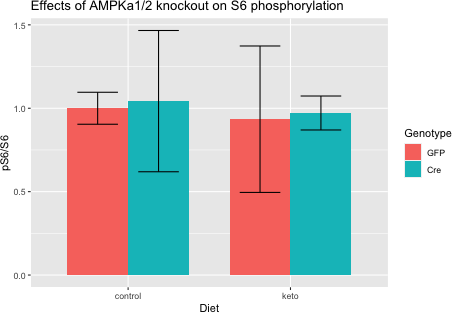
\includegraphics{figures/pS6-barplot-1.png}

\begin{longtable}[]{@{}lrrrrr@{}}
\caption{ANOVA for S6 phosphorylation, no interaction}\tabularnewline
\toprule
term & df & sumsq & meansq & statistic & p.value\tabularnewline
\midrule
\endfirsthead
\toprule
term & df & sumsq & meansq & statistic & p.value\tabularnewline
\midrule
\endhead
Diet & 1 & 0.726 & 0.726 & 0.058 & 0.815\tabularnewline
Genotype & 1 & 0.264 & 0.264 & 0.021 & 0.887\tabularnewline
Residuals & 10 & 125.354 & 12.535 & NA & NA\tabularnewline
\bottomrule
\end{longtable}

\begin{longtable}[]{@{}lrrrrr@{}}
\caption{ANOVA for S6 phosphorylation, with interaction}\tabularnewline
\toprule
term & df & sumsq & meansq & statistic & p.value\tabularnewline
\midrule
\endfirsthead
\toprule
term & df & sumsq & meansq & statistic & p.value\tabularnewline
\midrule
\endhead
Diet & 1 & 0.726 & 0.726 & 0.052 & 0.825\tabularnewline
Genotype & 1 & 0.264 & 0.264 & 0.019 & 0.893\tabularnewline
Diet:Genotype & 1 & 0.001 & 0.001 & 0.000 & 0.993\tabularnewline
Residuals & 9 & 125.353 & 13.928 & NA & NA\tabularnewline
\bottomrule
\end{longtable}

\hypertarget{integrated-stress-response}{%
\section{Integrated Stress Response}\label{integrated-stress-response}}

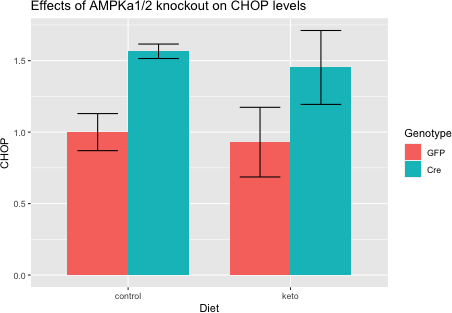
\includegraphics{figures/chop-barplot-1.png}

\begin{longtable}[]{@{}lrrrrr@{}}
\caption{ANOVA for CHOP levels, no interaction}\tabularnewline
\toprule
term & df & sumsq & meansq & statistic & p.value\tabularnewline
\midrule
\endfirsthead
\toprule
term & df & sumsq & meansq & statistic & p.value\tabularnewline
\midrule
\endhead
Diet & 1 & 0 & 0 & 0.075 & 0.790\tabularnewline
Genotype & 1 & 0 & 0 & 7.416 & 0.021\tabularnewline
Residuals & 10 & 0 & 0 & NA & NA\tabularnewline
\bottomrule
\end{longtable}

\begin{longtable}[]{@{}lrrrrr@{}}
\caption{ANOVA for CHOP levels, with interaction}\tabularnewline
\toprule
term & df & sumsq & meansq & statistic & p.value\tabularnewline
\midrule
\endfirsthead
\toprule
term & df & sumsq & meansq & statistic & p.value\tabularnewline
\midrule
\endhead
Diet & 1 & 0 & 0 & 0.067 & 0.801\tabularnewline
Genotype & 1 & 0 & 0 & 6.682 & 0.029\tabularnewline
Diet:Genotype & 1 & 0 & 0 & 0.010 & 0.921\tabularnewline
Residuals & 9 & 0 & 0 & NA & NA\tabularnewline
\bottomrule
\end{longtable}

\hypertarget{session-information}{%
\section{Session Information}\label{session-information}}

\begin{Shaded}
\begin{Highlighting}[]
\KeywordTok{sessionInfo}\NormalTok{()}
\end{Highlighting}
\end{Shaded}

\begin{verbatim}
## R version 4.0.0 (2020-04-24)
## Platform: x86_64-apple-darwin17.0 (64-bit)
## Running under: macOS Catalina 10.15.5
## 
## Matrix products: default
## BLAS:   /Library/Frameworks/R.framework/Versions/4.0/Resources/lib/libRblas.dylib
## LAPACK: /Library/Frameworks/R.framework/Versions/4.0/Resources/lib/libRlapack.dylib
## 
## locale:
## [1] en_US.UTF-8/en_US.UTF-8/en_US.UTF-8/C/en_US.UTF-8/en_US.UTF-8
## 
## attached base packages:
## [1] stats     graphics  grDevices utils     datasets  methods   base     
## 
## other attached packages:
## [1] broom_0.5.6   ggplot2_3.3.0 readxl_1.3.1  dplyr_0.8.5   tidyr_1.0.3  
## [6] knitr_1.28   
## 
## loaded via a namespace (and not attached):
##  [1] Rcpp_1.0.4.6     highr_0.8        plyr_1.8.6       pillar_1.4.4    
##  [5] compiler_4.0.0   cellranger_1.1.0 tools_4.0.0      digest_0.6.25   
##  [9] evaluate_0.14    lifecycle_0.2.0  tibble_3.0.1     gtable_0.3.0    
## [13] nlme_3.1-147     lattice_0.20-41  pkgconfig_2.0.3  rlang_0.4.6     
## [17] magick_2.3       yaml_2.2.1       xfun_0.13        withr_2.2.0     
## [21] stringr_1.4.0    generics_0.0.2   vctrs_0.2.4      grid_4.0.0      
## [25] tidyselect_1.0.0 glue_1.4.0       R6_2.4.1         rmarkdown_2.1   
## [29] purrr_0.3.4      farver_2.0.3     magrittr_1.5     backports_1.1.6 
## [33] scales_1.1.0     ellipsis_0.3.0   htmltools_0.4.0  assertthat_0.2.1
## [37] colorspace_1.4-1 labeling_0.3     stringi_1.4.6    munsell_0.5.0   
## [41] crayon_1.3.4
\end{verbatim}

\end{document}
